\documentclass[conference]{IEEEtran}
\IEEEoverridecommandlockouts

\usepackage{cite}
\usepackage{amsmath,amssymb,amsfonts}
\usepackage{algorithmic}
\usepackage{graphicx}
\usepackage{textcomp}
\usepackage{xcolor}
\def\BibTeX{{\rm B\kern-.05em{\sc i\kern-.025em b}\kern-.08em T\kern-.1667em\lower.7ex\hbox{E}\kern-.125emX}}
\usepackage{verbatimbox}

\begin{document}

\title{Multi-Objective Optimization in Image Approximation \\ {}
\thanks{The publication has been prepared with the support of Velbazhd Software LLC and Bulgarian Ministry of Education and Science according to the research project No. {D01–205/23.11.2018}.}}

\author{\IEEEauthorblockN{Plamen Petrov}
\IEEEauthorblockA{\textit{Institute of Information and Communication Technologies} \\
\textit{Bulgarian Academy of Sciences} \\
1113 Sofia, Bulgaria \\
p.petrov@iit.bas.bg}
\and
\IEEEauthorblockN{Georgi Kostadinov}
\IEEEauthorblockA{\textit{Institute of Information and Communication Technologies} \\
\textit{Bulgarian Academy of Sciences} \\
1113 Sofia, Bulgaria \\
g.kostadinov@iit.bas.bg}
\and
\IEEEauthorblockN{Petar Zhivkov}
\IEEEauthorblockA{\textit{Institute of Information and Communication Technologies} \\
\textit{Bulgarian Academy of Sciences} \\
1113 Sofia, Bulgaria \\
City, Country \\
pzhivkov@iit.bas.bg}
\and
\IEEEauthorblockN{Veneta Velichkova}
\IEEEauthorblockA{\textit{Institute of Information and Communication Technologies} \\
\textit{Bulgarian Academy of Sciences} \\
1113 Sofia, Bulgaria \\
vvelichkova@iit.bas.bg}
\and
\IEEEauthorblockN{Stoyan Ivanov}
\IEEEauthorblockA{\textit{Institute of Information and Communication Technologies} \\
\textit{Bulgarian Academy of Sciences} \\
1113 Sofia, Bulgaria \\
et\_idea@abv.bg}
\and
\IEEEauthorblockN{Todor Balabanov}
\IEEEauthorblockA{\textit{Institute of Information and Communication Technologies} \\
\textit{Bulgarian Academy of Sciences} \\
1113 Sofia, Bulgaria \\
0000-0003-3139-069X}
}

%
% Plamen Petrov - p.petrov@iit.bas.bg
% Georgi Kostadinov - g.kostadinov@iit.bas.bg
% Petar Zhivkov - pzhivkov@iit.bas.bg
% Veneta Velichkova - vvelichkova@iit.bas.bg
% Stoyan Ivanov - et_idea@abv.bg
% Todor Balabanov - todorb@iinf.bas.bg
%
% Bulgarian Academy of Sciences
% Institute of Information and Communication Technologies
% acad. Georgi Bonchev Str., block 2, office 514
% 1113 Sofia, Bulgaria
% http://iict.bas.bg/
%

\maketitle

\begin{abstract}
There are two common ways for the representation of images - as pixels (raster graphics) or as a list of geometric primitives (vector graphics). Both ways have their advantages and disadvantages and in some situations conversion between them is needed. Conversion from vector graphics to raster graphics is relatively easy and it is done by a process called rasterization. The opposite conversion (from raster to vector) is much harder and less reliable. The process is called vectorization and in the case of images, it is related to color reduction and information loss. The goal in this research is 16M colors bitmap images to be approximated with 12 colors vectorized form in which the base primitive is an ellipse. The process of vectorization is done with genetic algorithms as one of the most efficient metaheuristic tools for global optimization. The evaluation of the fitness value in the evolution process implemented in the genetic algorithms uses three different objective functions: 1) Average Euclidean distance between the pixels of the original image and the approximated image; 2) The size of the blanks spaces in the approximated image; and 3) The number of graphic primitives used for the approximation. 
\end{abstract}

\begin{IEEEkeywords}
image approximation, genetic algorithms, colors reduction, image vectorization
\end{IEEEkeywords}

\section{Introduction}

Packing problems are well known in geometry for centuries and there are even more relevant with the extensive development of soft computing \cite{Angelova-2009}. The goal is to pack certain objects into a container. The most popular case of this problem is when a single container should be filled as dense as possible \cite{Lodi-Martello-Monaci-2002}. There is a dualism for each packing problem as a covering problem. In covering problems it is asked how many objects are required in such organization that will cover the most area in the container. This problem is defined in two cases where object can or can not overlap. The most popular problems in two-dimensional space are: Packing circles in a circle \cite{Fodor-2003}; Packing circles in a square \cite{Huang-Ye-2010}; Packing circles in an isosceles or right triangle \cite{Xu-1996}; Packing circles an equilateral triangle \cite{Nurmela-2000}; Packing squares in a square \cite{Stromquist-2003}.

In this research, a multi-objective optimization with genetic algorithms is applied for a covering problem. The area to cover is rectangular and covering shapes are ellipses. They are of identical sizes. They should be placed on different coordinates and orientation angles. The final goal is a bitmap image to be transferred to G-Code instructions and acrylic paint to be drawn with a 2D plotting machine. 

After the introductory section, the paper is organized as follows: The second section defines the problem; The third section introduces some experiments and results; Finally, the fourth section concludes. 

\section{Problem Definition}

Some visualization devices (IoT for example \cite{Dineva-Atanasova-2019}) are not capable to handle a high number of colors. This is the case with 2D plotting machines. They have limited number of different colors. Also, different colors are handled consequently. It means that the device is doing only a single color in time and proper job scheduling is needed \cite{Borissova-Mustakerov-2015}. The other very important feature of the plotting devices is that they are operating with graphical primitives (lines, arcs, and other simple shapes). Such handling of the visual information is pretty different than what is used in pixel-based devices. If a bitmap image should be visualized on a 2D plotting machine the bitmap image should be transformed in a set of instructions (usually G-Codes) and the number of colors should be drastically reduced. This process has two common components -  color reduction and vectorization.

Bitmap images usually have much more information than it is needed for the visual interception. Because of this, a process for image simplification can be applied in such way that less informative elements to be reduced or completely removed. Meanwhile, the most informative elements are kept \cite{Ferreira-Fonseca-Jorge-Ramalho-2004}. Bitmap simplification is widely applied in different areas. It has major role in optical character recognition for example \cite{Wenyin-Dori-1999}. Conversion from vector graphics to bitmap is pretty stable, robust, and reliable, but this is not the case with the conversion in the opposite direction \cite{Tombre-Ah-Soon-Dosch-Masini-Tabbone-1999}. As an input to image simplification algorithm is digital photographs. The output of the simplification algorithm is stylized vector data. The goal of the simplification algorithm is to represent the original image with simple geometric regions.

\subsection{Multi-objective Optimization}

Genetic algorithms are chosen for the process of global optimization. Genetic algorithms are inspired by the natural process of evolution. The proposed by the genetic algorithms sub-optimal solutions are organized in population \cite{Balabanov-Sevova-Kolev-2019}. Each individual in the population is represented as a vector and it is called a chromosome. In many cases, the initial population is initialized with randomly generated chromosomes \cite{Balabanov-Barova-Keremedchiev-2016}, but for some problems like the problem presented in this research, the initial population is initialized according statistical estimation of the original bitmap image. Searching for a better sub-optimal solution in genetic algorithms is organized as epochs of evolution with the production of new generations. Each new generation appears after three basic operations - selection, crossover, and mutation \cite{Balabanov-Zankinski-Barova-2016}. The selection operator is the core of optimization convergence. The empirical expectation is that when better-fitted chromosomes are selected for offspring production the offspring would be even better \cite{Balabanov-Zankinski-Dobrinkova-2011}. The selection operator relies totally on the fitness value calculation. In this research, fitness value is calculated according to three components - bitmap images closeness, size of blank areas, and the number of primitive shapes used for image approximation. These three different optimization goals make this optimization problem a multi-objective problem.  

\subsection{Technical Implementation}

Ellipse with predefined width and height is selected as base 2D visual primitive for the approximation. Ellipse is appropriate because acrylic paint will be drawn with a small brush. It is accepted that each stroke with the brush will resemble an ellipse. Sharp lines or long rectangles are the other options, but they are less close to the shape of a single brush stroke. For simplicity in the current research, it is accepted that all ellipses are with identical sized. This can be elaborated on in some further researchers. Each ellipse is described with four numerical values - coordinates of the center (x and y values), angle of rotation around the center, and index of color from the provided list of colors. 

A list of ellipses with variable size presents the genetic algorithm chromosome. The list of ellipses is sorted before fitness value calculation because the most frequent colors should be drawn first and the less frequent colors should be drawn last. Such a drawing organization is needed because ellipses are allowed to overlap and the most frequent once can completely cover the least frequent once. The length of the chromosomes can vary and it is one of the criteria put under optimization. If the approximated image can be drawn with less number of primitive objects it will reduce drawing time (operating efficiency) and paint consumption (cost efficiency). 

The exploration part of genetic algorithms is done with the crossover operator. With chromosomes as lists of ellipses uniform crossover perfectly fits the need of exploration. Getting elements from parent chromosomes is organized in such way that children can be produced with different lengths. The exploitation part of genetic algorithms is done with the mutation operator. In this research randomly selected ellipse from the child chromosome is randomly changed as coordinates of the center, rotation angle, and color index. The trade-off between exploration and exploitation in genetic algorithms affects the completeness of wide optimization space investigation and near sub-optimal solutions investigation \cite{Hussain-Muhammad-2020}.

\begin{figure}[htbp]
\centerline{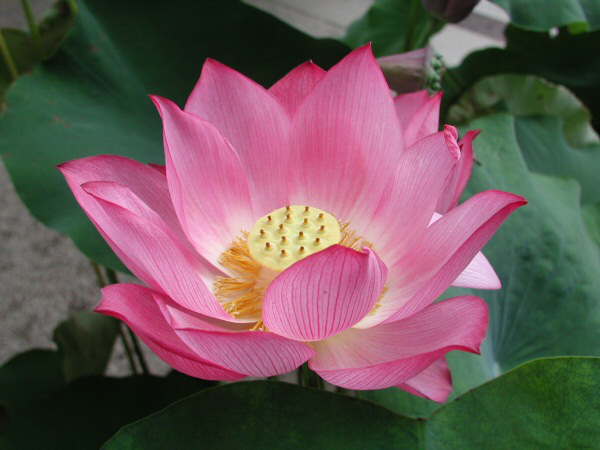
\includegraphics[width=0.5\textwidth]{fig01.png}}
\caption{Bitmap image used as an input.}
\label{fig01}
\end{figure}

The first component in the multi-objective fitness function is the closeness between the original bitmap image and the approximated bitmap image. As smaller is the difference between the both images as better is the sub-optimal solution. For this objective minimum is desired as sub-optimality. For the calculation of closeness, the original bitmap is taken unmodified. The approximated image on the other side is generated by drawing of all chromosome's ellipses in a bitmap image. Both images have identical dimensions. In the current research, the average Euclidean distance between the pixels in the images is calculated. Such a measure of image similarity is not accurate enough. It does not take into account image composition. In some further research, it will be better some kind of hierarchical granularity to be involved. 

The second component in the multi-objective fitness function is the total amount of blank area. The perfect case for this objective is when there is no blank area. As with the previous objective, the minimum is desired for better sub-optimality. The amount of blank area is easily calculated by filling the initial drawing area of the approximated image with a certain value of transparency. The amount of blank area is the count of the pixels which remain unchanged after ellipses drawing. 

The third component in the multi-objective fitness function is the count of drawn ellipses. It is obvious that less number of ellipses will faster produce a picture with less paint usage. As with the previous two objectives, the minimum is desired as a better sub-optimality. This objective dramatically opposes the other two objectives. If the number of drawn ellipses is zero it will not cost time and it will not cost paint. The problem is that with zero ellipses images distancing will be high and the blank area will be the maximum possible. 

A precise formulation of the problem is available in the public domain \cite{Balabanov-2020}. A precise description of the used genetic algorithm is available at \cite{Apache-Commons-Command-Line-Interface-2020}.

\section{Experiments \& Results}

All experiments are done on a single processor desktop machine - Intel Core i5, 2.3 GHz, 2 Cores, 8GB RAM and Mac OS X 10.13.6, Oracle Java 1.8.0-91. Experiments are organized as an open-source program written in Java especially for this research \cite{Balabanov-2020}. Apache Commons - Genetic Algorithms \cite{Apache-Commons-Genetic-Algorithms-2020} is used as a Java-based programming library for the optimization part of the program. Apache Commons - Command Line Interface \cite{Apache-Commons-Command-Line-Interface-2020} is used as a Java-based programming library for the program's input parameters handling.

The photograph shown in Fig. \ref{fig01} is used as an input for the experiments. A set of 12 basic colors is used for the output image, as follows:   FFFFFF (White), FFFF00 (Yellow), CC7722 (Ochre), E34234 (Vermillon), DC143C(Crimson), 49796B (Hooker's Green), 40826D (Viridian), 120A8F (Ultramarine Blu), 0000FF (Coblat Blue), E97451 (Burnt Sienna), 635147 (Raw Umber), 000000 (Black). On a trial and error bases, 37 individuals are chosen for the size of the population. The arity of tournament selection is chosen to be 2. The crossover rate is chosen to be 95\%. The mutation rate is chosen to be 1\%. The elitism rule is applied for 5\% of the population. Time limit of one hour is chosen for stopping criteria.

\begin{figure}[htbp]
\centerline{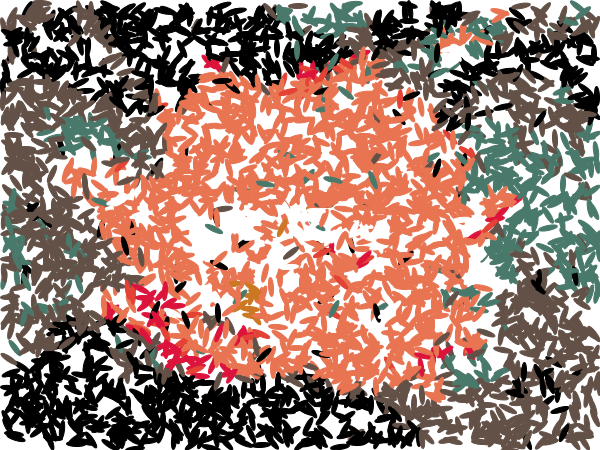
\includegraphics[width=0.5\textwidth]{fig02.png}}
\caption{The result after the first run of the experiment.}
\label{fig02}
\end{figure}

\begin{figure}[htbp]
\centerline{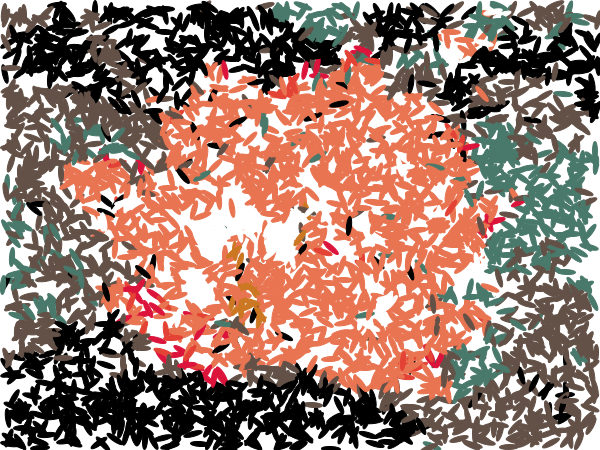
\includegraphics[width=0.5\textwidth]{fig03.png}}
\caption{The result after the second run of the experiment.}
\label{fig03}
\end{figure}

\begin{figure}[htbp]
\centerline{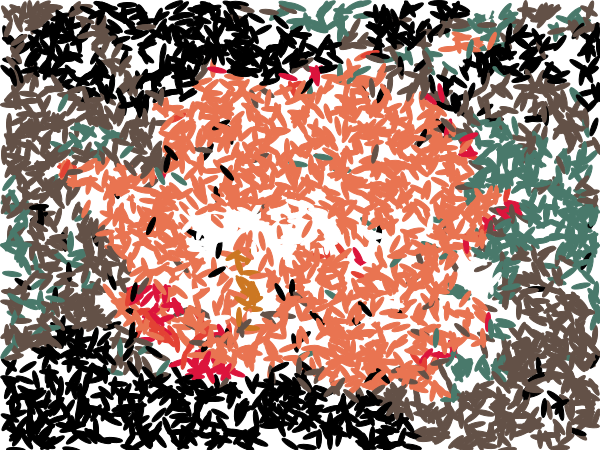
\includegraphics[width=0.5\textwidth]{fig04.png}}
\caption{The result after the third run of the experiment.}
\label{fig04}
\end{figure}

\begin{figure}[htbp]
\centerline{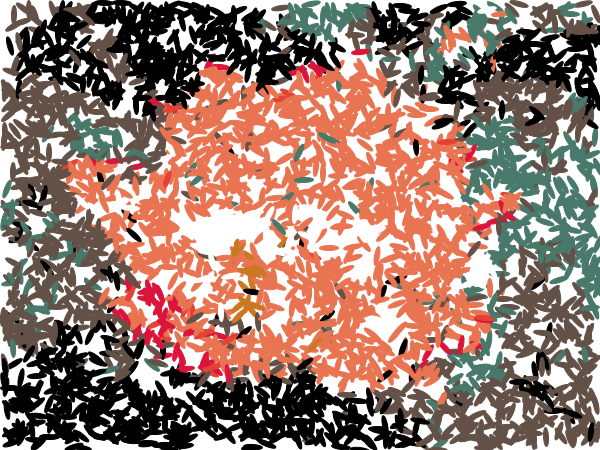
\includegraphics[width=0.5\textwidth]{fig05.png}}
\caption{The result after the fourth run of the experiment.}
\label{fig05}
\end{figure}

\begin{figure}[htbp]
\centerline{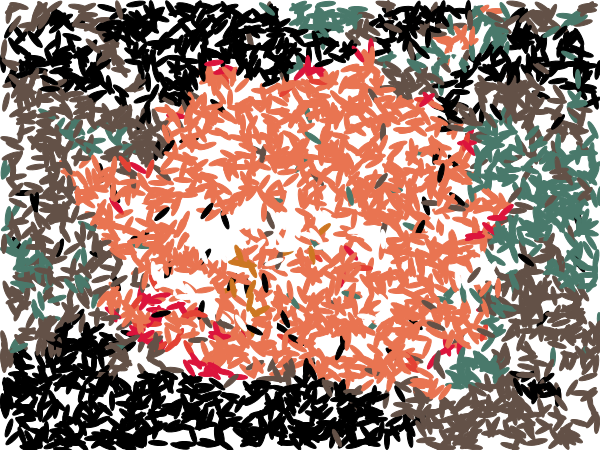
\includegraphics[width=0.5\textwidth]{fig06.png}}
\caption{The result after the fifth run of the experiment.}
\label{fig06}
\end{figure}

\begin{figure}[htbp]
\centerline{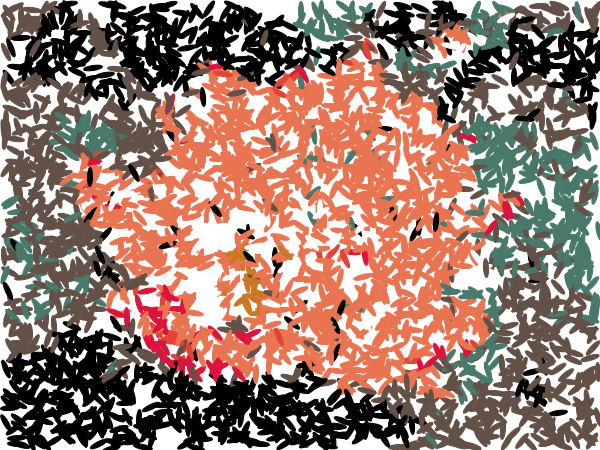
\includegraphics[width=0.5\textwidth]{fig07.png}}
\caption{The result after the sixth run of the experiment.}
\label{fig07}
\end{figure}

Parameters used for the optimization are as follows:

\begin{verbnobox}[\small]
java -jar Ellipses-Image-Approximator-all.jar 
-input ../../input/0001.jpg -output ~/Desktop/ 
-pixel_closest_color -g_code_print 
-g_code_comments -g_code_x_home 40 
-g_code_y_home 90 -g_code_z_up 35 
-g_code_z_down 80 -g_code_width 80.0 
-g_code_height 80.0 -g_code_refill_count 3 
-ellipse_width 19 -ellipse_height 5 
-ellipse_alpha 216 -colors FFFFFF,FFFF00,
CC7722,E34234,DC143C,49796B,40826D,
120A8F,0000FF,E97451,635147,000000 -ga 
-ga_population_size 37 -ga_tournament_arity 2 
-ga_crossover_rate 0.95 -ga_mutation_rate 0.01 
-ga_elitism_rate 0.05 -ga_optimization_time 3600
\end{verbnobox}

Six separate experiments were executed. As it is shown in Fig. \ref{fig02}-\ref{fig07}, the most informative elements of the bitmap image are kept in the approximated images. There are some deviations in the results, but it is expected because of the probabilistic nature of the genetic algorithms. The number of the ellipses used for the approximation is acceptable (if the number is too high it will be time and paint consuming), but the presence of obvious blank areas is not of the desired amount. Each interested reader can try different genetic algorithm parameters with different images of his/her own choice, because of the implemented command-line interface. 

\section{Conclusion}

In this paper, multi-objective optimization was proposed for image approximation. As an optimization tool, genetic algorithms are used. The experimental results clearly show that approximated images are perception close with the limitation of color reduction and vectorization. The convergence of the optimization process is very related to the probabilistic nature of the genetic algorithms. Because of this, the implementation of an efficient fitness function is critical in the process. The main disadvantage of the proposed solution is the time-consuming raster image cooperation. 

As further research, it will be challenging distributed genetic algorithms to be applied. In such implementation, the most time-consuming calculations would be done on different heterogeneous machines or on a single supercomputer as AVITOHOL \cite{Tashev-Tasheva-Petrov-2019}. 

\section*{Acknowledgment}

This research is funded by Velbazhd Software LLC and it is partially supported by the Bulgarian Ministry of Education and Science (contract D01–205/23.11.2018) under the National Scientific Program ``Information and Communication Technologies for a Single Digital Market in Science, Education and Security (ICTinSES)'', approved by DCM \# 577/17.08.2018.

\begin{thebibliography}{00}

\bibitem{Angelova-2009} V. Angelova, ``Investigations in the Area of Soft Computing Targeted State of the Art Report'', Cybernetics and Information Technologies, vol. 9, no. 1, 2009, pp. 18--24.

\bibitem{Lodi-Martello-Monaci-2002} A. Lodi, S. Martello, M. Monaci, ``Two-dimensional packing problems: A survey'', European Journal of Operational Research (Elsevier), vol. 141, no. 2, 2002, pp. 241--252.

\bibitem{Fodor-2003} F. Fodor, ``The Densest Packing of 13 Congruent Circles in a Circle'', Beitrage zur Algebra und Geometrie, Contributions to Algebra and Geometry, vol. 44, no. 2, 2003, pp. 431--440.

\bibitem{Huang-Ye-2010} W. Huang, T. Ye, ``Greedy vacancy search algorithm for packing equal circles in a square'', Operations Research Letters, vol. 38, 2010, pp. 378--382.

\bibitem{Xu-1996} Y. Xu, ``On the minimum distance determined by n ($<$= 7) points in an isoscele right triangle'', Acta Mathematicae Applicatae Sinica, vol. 12, no. 2, 1996, pp. 169--175.

\bibitem{Nurmela-2000} K. Nurmela, ``Conjecturally optimal coverings of an equilateral triangle with up to 36 equal circles'', Experimental Mathematics, vol. 9, no. 2, 2000, pp. 241--250.

\bibitem{Stromquist-2003} W. Stromquist, ``Packing 10 or 11 unit squares in a square'', Electronic Journal of Combinatorics, vol. 10, no. 8, 2003, pp. 1--11.

\bibitem{Dineva-Atanasova-2019} K. Dineva, T. Atanasova, ``Methodology for Data Processing in Modular IoT System'', Distributed Computer and Communication Networks, Proceedings of 22-st International Conference, Springer Nature Switzerland, vol. 11965, 2019, pp. 457--468.

\bibitem{Borissova-Mustakerov-2015} D. Borissova, I. Mustakerov, ``Open job shop scheduling via enumerative combinatorics'', International Journal of Mathematical Models and Methods in Applied Sciences, vol. 9, 2015, pp. 120--127.

\bibitem{Ferreira-Fonseca-Jorge-Ramalho-2004} A. Ferreira, M.J. Fonseca, J.A.Jorge, M. Ramalho, ``Mixing Images and Sketches for Retrieving Vector Drawings'', The 7th Eurographics Workshop on Multimedia (EGMM04), China, 2004.

\bibitem{Wenyin-Dori-1999} L. Wenyin, D. Dori, ``From Raster to Vectors: Extracting Visual Information from Line Drawings'', Pattern Analysis and Applications (PAA), 1999.

\bibitem{Tombre-Ah-Soon-Dosch-Masini-Tabbone-1999} K. Tombre, C. Ah-Soon, P. Dosch, G. Masini, S. Tabbone, ``Stable and robust vectorization: How to make the right choices'', Proceedings of the 3rd IAPR Intlernational Workshop on Graphics Recognition, Jaipur, India, 1999, pp. 3--16.

\bibitem{Balabanov-Sevova-Kolev-2019} T. Balabanov, J. Sevova, K. Kolev, ``Optimization of String Rewriting Operations for 3D Fractal Generation with Genetic Algorithms'', Proceedings of International Conference on Numerical Methods and Applications, Lecture Notes in Computer Science, vol. 11189, 2019, pp. 48--54.

\bibitem{Balabanov-Barova-Keremedchiev-2016} T. Balabanov, M. Barova, D. Keremedchiev, ``Image Construction with 2D Ellipses by Genetic Algorithms Optimization'', Abstracts of Annual Meeting of the Bulgarian Section of SIAM, Fastumprint, 2016, pp. 10--11.

\bibitem{Balabanov-Zankinski-Barova-2016} T. Balabanov, I. Zankinski, M. Barova, ``Strategy for Individuals Distribution by Incident Nodes Participation in Star Topology of Distributed Evolutionary Algorithms'', Cybernetics and Information Technologies, vol. 16, no. 1, 2016, pp. 80--88.

\bibitem{Balabanov-Zankinski-Dobrinkova-2011} T. Balabanov, I. Zankinski, N. Dobrinkova, ``Time Series Prediction by Artificial Neural Networks and Differential Evolution in Distributed Environment'', Proceedings of International Conference on Large-Scale Scientific Computing, Lecture Notes in Computer Science, vol. 7116, 2011, pp. 198--205.

\bibitem{Hussain-Muhammad-2020} A. Hussain, Y.S. Muhammad, ``Trade-off between exploration and exploitation with genetic algorithm using a novel selection operator'', Complex \& Intelligent Systems, vol. 6, 2020, pp. 1--14.

\bibitem{Balabanov-2020} T. Balabanov, ``Ellipses Image Approximator'', http://github.com/TodorBalabanov/EllipsesImageApproximator/

\bibitem{Apache-Commons-Genetic-Algorithms-2020} ``Apache Commons - Genetic Algorithms'', http://commons.apache.org/proper/commons-math/userguide/genetics.html

\bibitem{Apache-Commons-Command-Line-Interface-2020} ``Apache Commons - Command Line Interface'', http://commons.apache.org/proper/commons-cli/

\bibitem{Tashev-Tasheva-Petrov-2019} T. Tashev, R. Tasheva, P. Petrov, ``Determination of the Computer Modelling Precision for Throughput of Switch Node with LPF-algorithm'', Proceedings of  International Conference on Computer Systems and Technologies, ACM, 2019, pp. 141--145.

\end{thebibliography}

\end{document}
